\subsection{Entidad \textit{Ascensor}:} \label{bloque:Ascensor}
    Esta entidad engloba el funcionamiento del ascensor al completo, será la última etapa y la que se sintetizará sobre la FPGA.\\

    La interfaz, entradas y salidas, de este bloque se puede ver su representación en la Figura \ref{fig:EntidadIAscensor}:
    
    \begin{figure}[H]
		    \centering
		    \includegraphics[width = 0.8\textwidth ]{EntidadAscensor}
		    \caption{Diagrama de la Interfaz de la Entidad Ascensor}
		    \label{fig:EntidadIAscensor}
	\end{figure}
	
	Esta es una entidad de alto nivel que encapsula todo el funcionamiento del ascensor. Se puede ver el diagrama de bloques interno de esta entidad en la siguiente figura: 
	
	\begin{figure}[H]
		    \centering
		    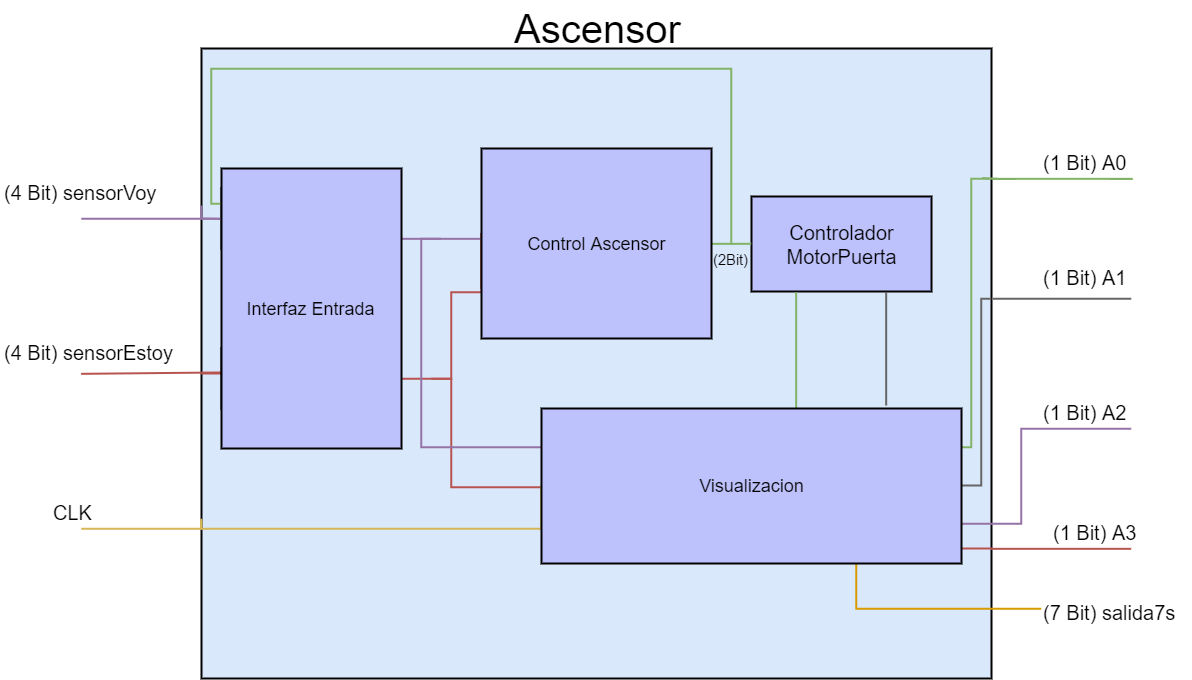
\includegraphics[width = .85\textwidth ]{EntidadAscensorEntidades}
		    \caption{Diagrama interno de la entidad Ascensor}
		    \label{fig:EntidadIAscensorEntidades}
	\end{figure}
	
	Como se puede ver en la figura anterior se han encapsulado los bloques en diferentes entidades en función de su finalidad, estas entidades se pueden ver a continuación. En las representaciones de estas entidades se verá que hay ciertos bloques repetidos, se trata del mismo bloque utilizado dos veces, no de bloques diferentes, que se han representado por duplicado para mayor claridad. \\ 

	Se adelanta el esquema del funcionamiento general del ascensor (obviando las entidades generales):

	\begin{figure}[H]
		    \centering
		    \includegraphics[width = .85\textwidth ]{EntidadAscensorInterior}
		    \caption{Diagrama funcionamiento del Ascensor}
		    \label{fig:EntidadIAscensorInterior}
	\end{figure}

\subsection{Entidad \textit{Interfaz Entrada}:} \label{bloque:InterfazEntrada}
	Esta entidad se encarga de gestionar los datos de las entradas para adaptarlos al funcionamiento interno de nuestro sistema, en este caso se encarga de codificar y modular correctamente las señales de los sensores del piso al que voy y del piso en que estoy. \\ 

	Como se ve en la figura (\ref{fig:EntidadesAscensorE1}), engloba dos bloques, que se describen en los siguientes apartados.
	\begin{figure}[H]
		    \centering
		    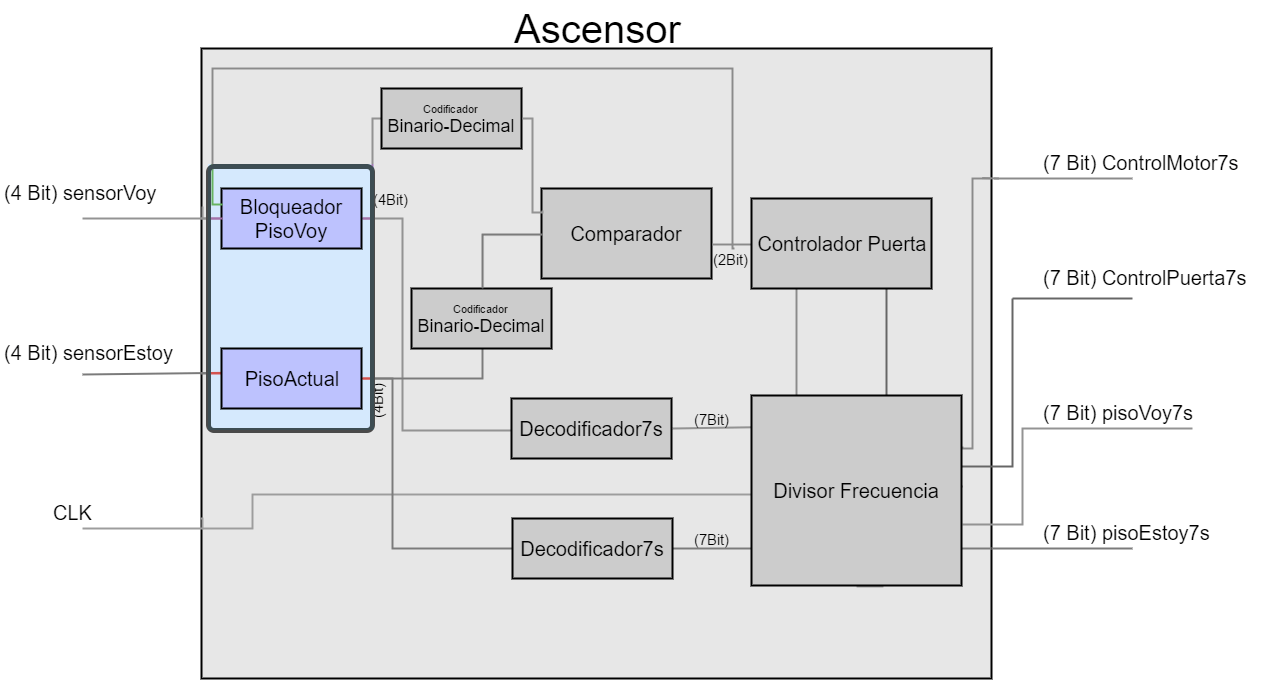
\includegraphics[width = .85\textwidth ]{EntidadAscensorInterior(E1)}
		    \caption{Representación de la Entidad Interfaz Entrada}
		    \label{fig:EntidadesAscensorE1}
	\end{figure}

	Se puede ver en la figura (\ref{fig:EntidadInterfazEntrada}) que este bloque tiene tres entradas, las lecturas del piso actual y el piso objetivo y el reloj que utilizaremos para hacer síncrono el proceso. Y cuatro salidas, todas ellas vectores de 4 bits, que almacenan las lecturas válidas de los sensores.
	\begin{figure}[H]
		    \centering
		    \includegraphics[width = .85\textwidth ]{EntidadInterfazEntrada}
		    \caption{Diagrama de la Interfaz de la Entidad Interfaz Entrada}
		    \label{fig:EntidadInterfazEntrada}
	\end{figure}

\subsection{Entidad \textit{Control Ascensor}:} \label{bloque:ControlAscensor}
	Esta entidad se encarga de gestionar el funcionamiento del ascensor propiamente dicho comparando las lecturas de los sensores y decidiendo que deben hacer los actuadores, el motor y la puerta.  \\ 

	Como se ve en la figura (\ref{fig:EntidadesAscensorE3}), engloba tres bloques, que se explican más adelante. Según se puede observar el bloque Codigicador Binario-Decimal se utiliza dos veces.
	\begin{figure}[H]
		    \centering
		    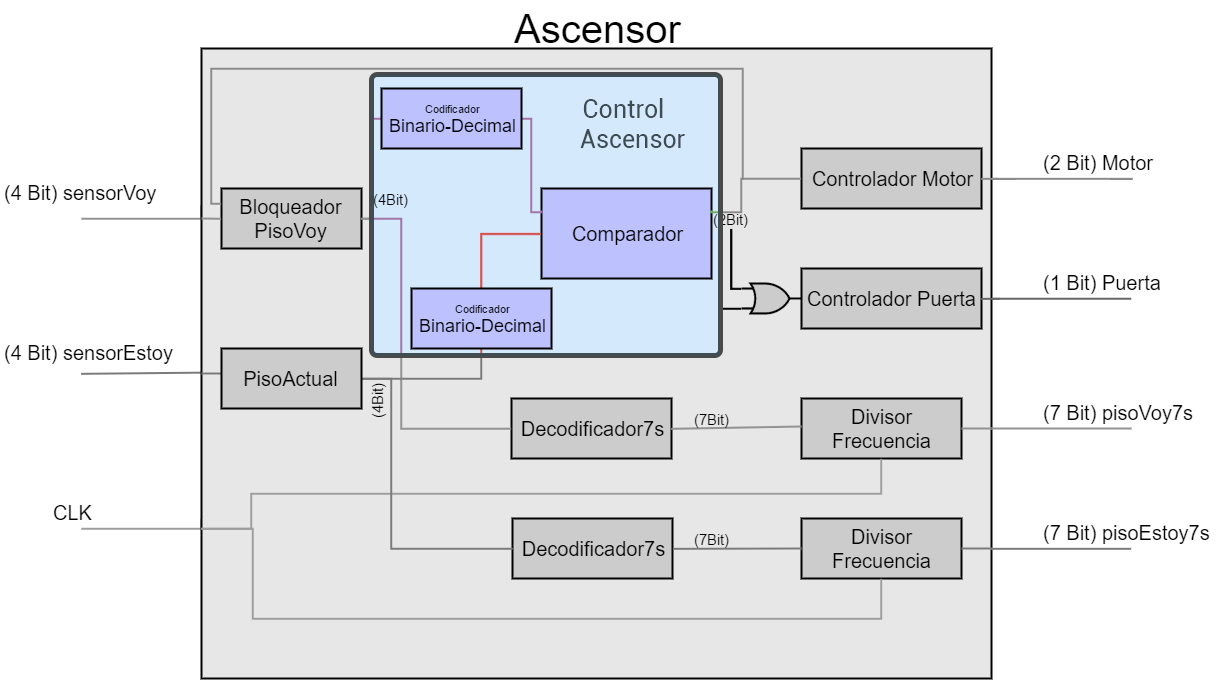
\includegraphics[width = .85\textwidth ]{EntidadAscensorInterior(E3)}
		    \caption{Representación de la Entidad Control Ascensor}
		    \label{fig:EntidadesAscensorE3}
	\end{figure}

	Se puede ver en la figura (\ref{fig:EntidadControlAscensor}) que este bloque tiene tres entradas, las lecturas del piso actual y el piso objetivo y el reloj que utilizaremos para hacer síncrono el proceso. Y que tras compararlas se obtiene una salida, que codifica la accción que realizarán tanto el motor como la puerta.
    \begin{figure}[H]
		    \centering
		    \includegraphics[width = .85\textwidth ]{EntidadControlAscensor}
		    \caption{Diagrama de la Interfaz de la Entidad Control Ascensor}
		    \label{fig:EntidadControlAscensor}
	\end{figure} 

\subsection{Entidad \textit{Visualizacion}:} \label{bloque:Visualizacion}	
	Esta entidad se encarga de gestionar la salida visual de los datos a través de los display de 7 segmentos. Para ello codifica dichas señales a los 7 bits del display para luego, mediante un alternador de displays ir alternando cada display de forma que en cada uno de los cuatro se muestre la información debida.  \\ 

	Como se ve en la figura (\ref{fig:EntidadesAscensorE2}), engloba cuatro bloques bloques, que se detallan en apartados posteriores. Según se puede observar el bloque Decodificador7s se utiliza dos veces.
	\begin{figure}[H]
		    \centering
		    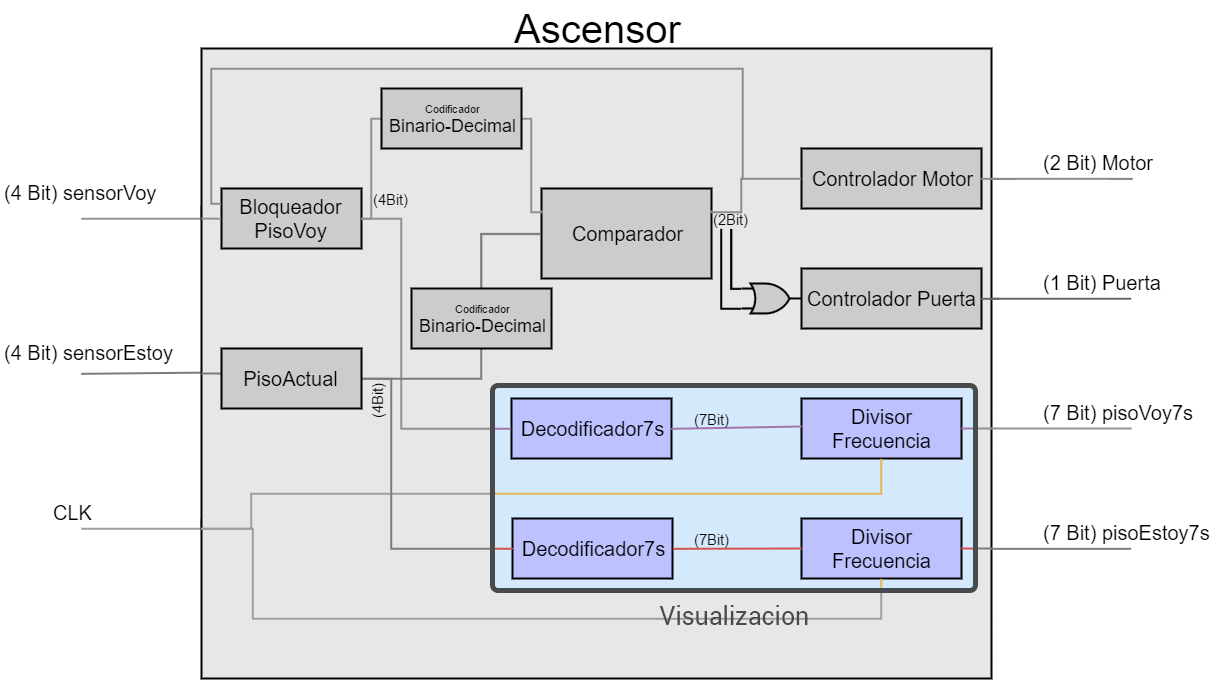
\includegraphics[width = .85\textwidth ]{EntidadAscensorInterior(E2)}
		    \caption{Representación de la Entidad Visualizacion}
		    \label{fig:EntidadesAscensorE2}
	\end{figure}

	Se puede ver en la figura (\ref{fig:EntidadVisualizacion}) que este bloque tiene cinco entradas, estado del motor, estado de la puerta, el piso actual, el piso destino y el reloj que utilizaremos para hacer síncrono el proceso. Y las cinco salidas necesarias para mostrar los datos en el display.
    \begin{figure}[H]
		    \centering
		    \includegraphics[width = .85\textwidth ]{EntidadVisualizacion}
		    \caption{Diagrama de la Interfaz de la Entidad Visualizacion}
		    \label{fig:EntidadVisualizacion}
	\end{figure} 


\subsection{Bloque \textit{Decodificador a 7 segmentos}:} \label{bloque:Decodificador7s}
    Este bloque es el encargado de traducir el piso en el que se encuentra el ascensor y el piso objetivo para poder mostrarlo en el display de 7 segmentos. Para ello es importante recordar el Cuadro (\ref{tab:tabla1ApendiceA}) del Apéndice \ref{app:codEntSal} donde podemos ver como se codifica internamente el número de piso. \\ 
    
    La salida que se verá en el display para cada caso se puede ver en la figura siguiente:
    
    \begin{figure}[H]
		    \centering
		    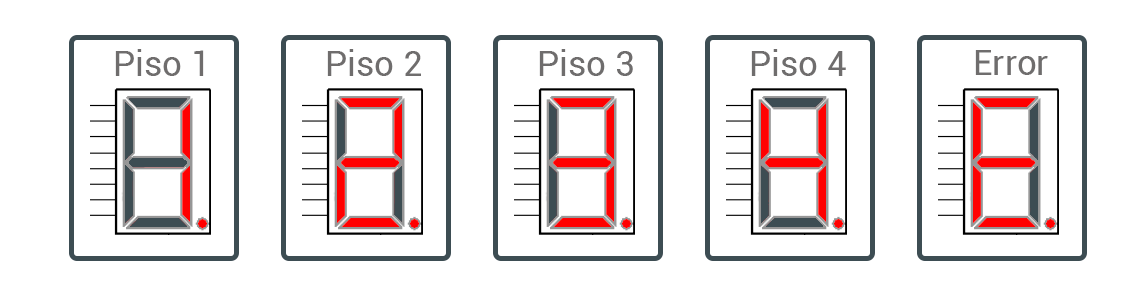
\includegraphics[width = 1\textwidth ]{displays7s}
		    \caption{Salida en los displays de 7 segmentos}
		    \label{fig:displays7s}
	\end{figure}
    
    La interfaz, entradas y salidas, de este bloque se puede ver su representación en la Figura \ref{fig:BloqueDecodificador7seg}. Como se ve entra la lecura del piso objetivo o el piso actual de 4 bits y sale la representación del caracter correspondiente en una señal de 7 bits:
    
    \begin{figure}[H]
		    \centering
		    \includegraphics[width = 0.7\textwidth ]{BloqueDecodificador}
		    \caption{Diagrama Interfaz Bloque Decodificador a 7 segmentos}
		    \label{fig:BloqueDecodificador7seg}
	\end{figure}
\subsection{Bloque \textit{Alternador de displays}:} \label{bloque:AlternadorDisplay}
    Este bloque es el encargado de gestionar la salida del Display alternando de un digito a otro de forma que en cada uno se muestre la información debida, debemos (dividir la frecuencia de reloj entre los cuatro dígitos). \\
    
	Como se ha dicho anteriormente cada digito debe contener 8 segmentos (pines de control), del segmento 7 al 1 son de las diferentes partes del digito y el último segmento (0) es el pin que controla el punto (dp) del digito, activos a nivel bajo. El pin que selecciona el digito que muestra en cada momento (ánodo de control) es activo a nivel alto. \\
	
	Como se puede apreciar en el siguiente diagrama la interfaz de este bloque tiene cinco entradas, 4 vectores de 7 bits, que contienen la información a mostrar  y un reloj que utilizaremos para hacer síncrono el proceso. Y cinco salidas, cuatro de ellas son enteros que indican cual es el digito a revelar y un vector de 4 bits, que codifica la información a mostrar del digito elegido.

	\begin{figure}[H]
		    \centering
		    \includegraphics[width = 0.7\textwidth ]{BloqueAlternadorDisplay}
		    \caption{Diagrama Interfaz Bloque Alternador Displays}
		    \label{fig:BloqueAlternadorDisplay}
	\end{figure}

\subsection{Bloque \textit{PisoActual}:} \label{bloque:PisoActual}
    Como se ha dicho anteriormente en cada piso hay un final de carrera que detecta el paso del ascensor. El propósito de este bloque es el de filtrar dicha entrada de 4 bits. En este caso lo que interesa es saber en que piso estoy o en que piso he estado por última vez. Cuando el ascensor se encuentra entre dos pisos la entrada de los sensores será \textit{0000}, este bloque lo que hará será mantener en la salida del mismo el último piso por el que haya pasado el ascensor. \\ 
    
    Como se puede apreciar en el siguiente diagrama este bloque tiene una entrada, un vector de 4 bits (los finales de carrera de cada piso) y una salida, también de 4 bits, codificando el piso en el que se encuentra actualmente. \\ 
    
    Se puede consultar dicha codificación en el Cuadro (\ref{tab:tabla1ApendiceA}) del Apéndice \ref{app:codEntSal}. \\ 
    
    La interfaz, entradas y salidas, de este bloque se puede ver su representación en la Figura \ref{fig:BloquePisoActual}:
    
    \begin{figure}[H]
		    \centering
		    \hspace*{-1.8cm}
		    \includegraphics[width = 0.6\textwidth ]{BloquePisoActual}
		    \caption{Diagrama Bloque PisoActual}
		    \label{fig:BloquePisoActual}
	\end{figure}
	
	Se puede consultar el código VHDL de este módulo en el Apartado \ref{code:PisoActual} así como el código de su testbench correspondiente en el Apartado \ref{code:PisoActual_tb}.\\ 

\subsection{Bloque \textit{Bloqueador PisoVoy}:} \label{bloque:BloqueadorPisoVoy}
    Mediante 4 interruptores (uno por planta) se ha codificado la llamada al ascensor, indicando a que piso debe ir el ascensor. La finalidad de este bloque es filtrar dicha entrada de 4 bits, nos interesa saber a qué piso debe ir el ascensor o a que piso ha ido por última vez. Pudiendo almacenar hasta tres pisos, a los que debe ir, en orden y parando un tiempo antes de ir al siguiente piso almacenado. \\
    
	Como se puede apreciar en el siguiente diagrama este bloque tiene tres entradas, un vector de 4 bits (los botones de cada piso), un vector de 2 bits (estado del motor) y el reloj que utilizaremos para hacer síncrono el proceso. Y tres salidas, vectores de 4 bits, codificando el piso al que debe ir el ascensor (PisoVoy) y dos pisos almacenados en las variables auxiliares (MemPisoVoy1 y MemPisoVoy2), codificando los piso a los que el usuario desea ir. \\
	
	Se puede consultar dicha codificación en el Cuadro (\ref{tab:tabla1ApendiceA}) del Apéndice \ref{app:codEntSal}. \\
    
    La interfaz, entradas y salidas, de este bloque se puede ver su representación en la Figura \ref{fig:BloqueBloqueadorPisoVoy}:
    
    \begin{figure}[H]
		    \centering
		    \hspace*{-1.8cm}
		    \includegraphics[width = 0.6\textwidth ]{BloqueBloqueadorPisoVoy}
		    \caption{Diagrama Bloque Bloqueador PisoVoy}
		    \label{fig:BloqueBloqueadorPisoVoy}
	\end{figure}
	
\subsection{Bloque \textit{Decodificador Binario a Entero}:} \label{bloque:DecodificadorBinarioEntero}
	En este bloque se traduce la señal binaria que codifica tanto el piso actual como el piso de destino a decimal para su posterior comparación.
	Se puede consultar dicha codificación en el Cuadro (\ref{tab:tabla1ApendiceA}) del Apéndice \ref{app:codEntSal}. \\ 

	Como se ve en la figura (\ref{fig:BloqueDecodificadorBinarioEntero}) este bloque tiene una entrada de 4 bits (codificación en binario) y una salida de 32bits, para la codificación como número entero.
	\begin{figure}[H]
		    \centering
		    \includegraphics[width = .85\textwidth ]{BloqueDecodificadorBinarioEntero}
		    \caption{Representación del bloque DecodificadorBinarioEntero}
		    \label{fig:BloqueDecodificadorBinarioEntero}
	\end{figure}

\subsection{Bloque \textit{Comparador}:} \label{bloque:Comparador}

	En este bloque es donde se deciden las acciones del ascensor. Para ello se introducen dos señales, dos números enteros (correspondientes al piso actual y al piso objetivo) y se comparan para dar una salida, que determinará la reacción del ascensor (puerta y motor). El reloj lo empleamos para sincronizar el proceso. \\ 

    La interfaz, entradas y salidas, de este bloque se puede ver su representación en la Figura \ref{fig:BloqueComparador}:
    
    \begin{figure}[H]
		    \centering
		    \includegraphics[width = 0.6\textwidth ]{BloqueComparador}
		    \caption{Diagrama Bloque Comparador}
		    \label{fig:BloqueComparador}
	\end{figure}



\subsection{Bloque \textit{Controlador Motor} y \textit{Controlador Puerta}:} \label{bloque:MotorPuerta}
    
    En este caso no tenemos ni puerta ni motor físico así que se ha decidido sacar la reacción que tendrían estos elementos por dos de los display de 7 segmentos de que se dispone. Este bloque se encarga de recibir la señal de dos bits que codifica la decisión del comparador (como se mueve el motor y que hace la puerta) y saca dos señales de 7 bits donde codifica el caracter que se mostrará en cada caso. Se puede ver el esquema en la figura (\ref{fig:MotorPuerta}). Se podrá ver en los displays los siguientes caracteres:\\ 

	\begin{table}[H]
        \centering
			\begin{tabular}{|ccccc|}
				\hline
				\rowcolor[rgb]{0.21,0.69,0.87}\multicolumn{3}{|c|}{  \textbf{ {Funcionamiento Motor}}} & \multicolumn{2}{|c|}{  \textbf{ {Funcionamiento Puerta}}} \\
				\hline \hline
				\hline
				 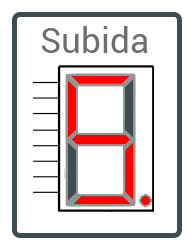
\includegraphics[width = 0.15\textwidth ]{CodCaracteres7s/subida} &  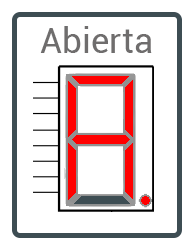
\includegraphics[width = 0.15\textwidth ]{CodCaracteres7s/abierta}  &
				 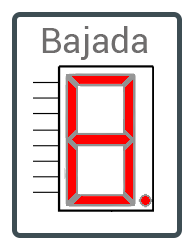
\includegraphics[width = 0.15\textwidth ]{CodCaracteres7s/bajada} &  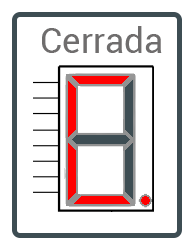
\includegraphics[width = 0.15\textwidth ]{CodCaracteres7s/Cerrada}  &
				 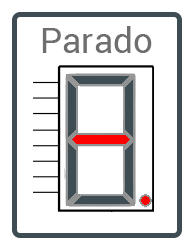
\includegraphics[width = 0.15\textwidth ]{CodCaracteres7s/parado}  \\
				\hline				 
			\end{tabular}
			\caption{ Salida en displays 7 segmentos para el control del motor y de la puerta }
			\label{tab:tablaVisualizacionMotorPuerta}
	\end{table}

	\begin{figure}[H]
		    \centering
		    \includegraphics[width = .85\textwidth ]{BloqueMotorPuerta}
		    \caption{Representación del bloque MotorPuerta}
		    \label{fig:MotorPuerta}
	\end{figure}

	La interfaz, entradas y salidas, de este bloque se puede ver su representación en la Figura \ref{fig:BloqueMotorPuerta}:
    
    \begin{figure}[H]
		    \centering
		    \includegraphics[width = 0.6\textwidth ]{BloqueMotorPuerta}
		    \caption{Diagrama Bloque Motor-Puerta}
		    \label{fig:BloqueMotorPuerta}
	\end{figure}

\subsection {Bloque \textit{DecodificadorLED} :} \label{bloque:DecodificadorLED}
    Este bloque se encarga de gestionar la salida de los leds. Usaremos los 8 leds de la placa, mostrando así dos pisos almacenados codificados según indicamos en el Cuadro (\ref{tab:tabla1ApendiceA}) del Apéndice \ref{app:codEntSal}. \\
    
	Como se puede apreciar en el siguiente diagrama este bloque tiene tres entradas, dos vectores de 4 bits (dos pisos diferentes) y un reloj que utilizaremos para hacer síncrono el proceso. \\ 
	
	Y una salida, un vector de 8 bits, que indica los leds que debe encender. Los cuatro bits de la derecha corresponden al primer piso almacenado y los otros cuatro al último piso almacenado. \\ 
    
	La interfaz, entradas y salidas, de este bloque se puede ver su representación en la Figura \ref{fig:BloqueDecodificadorLED}:
    
    \begin{figure}[H]
		    \centering
		    \includegraphics[width = 0.6\textwidth ]{BloqueDecodificadorLED}
		    \caption{Diagrama Bloque BloqueDecodificadorLED}
		    \label{fig:BloqueDecodificadorLED}
	\end{figure}
